\documentclass[10pt, aspectratio=1610]{beamer}

\usetheme{metropolis}
\usepackage[utf8]{inputenc}
\usepackage{amsmath}
\usepackage{amsfonts}
\usepackage{amssymb}
\usepackage{graphicx}
%\author{}
%\title{}
%\setbeamercovered{transparent} 
%\setbeamertemplate{navigation symbols}{} 
%\logo{} 
%\institute{} 
%\date{} 
%\subject{} 
\begin{document}

%\begin{frame}
%\titlepage
%\end{frame}

\begin{frame}{Inclusive jet cross section at small $R$}
\begin{eqnarray}
\frac{d\sigma}{dp_T} &=& \int_0^1 \frac{dz}{z} \frac{d\hat{\sigma}}{dq_T}(\frac{p_T}{z}, \mu) \mathcal{J}(z,\mu, \mu_J),~~\mu\sim p_T,~~\mu_J\sim p_T R\\
\hat{\sigma} &=& \hat{\sigma}^{(0)} + \hat{\sigma}^{(1)} + \cdots,~~~\mathcal{J} = \mathcal{J}^{(0)} + \mathcal{J}^{(1)} + \cdots
\end{eqnarray}
Achieve NLO accuracy of hard partonic cross-section $\hat{\sigma}$, and Leading-log (LL) accuracy of the evolved jet function $\mathcal{J}$ in vacuum and medium.
\begin{eqnarray}
\sigma = \underbrace{\hat{\sigma}^{(0)} \otimes \mathcal{J}^{(0)}}_{LO+LL}  +  \underbrace{\left(\hat{\sigma}^{(0)} \otimes \mathcal{J}^{(1)} + {\color{red}\hat{\sigma}^{(1)}} \otimes \mathcal{J}^{(0)}
\right)}_{NLO+LL} + \cdots
\end{eqnarray}
\begin{itemize}
\item NLO partonic cross section: see NPB327(1989)105-143, NPB539(1999)455-476, PRD86(2012)094009
\item Semi-inclusvie jet function: see JHEP10(2016)125 (light jet), JHEP07(2019)148 (heavy jet).
\end{itemize}
\end{frame}


\begin{frame}{The vacuum jet function}

\begin{center}
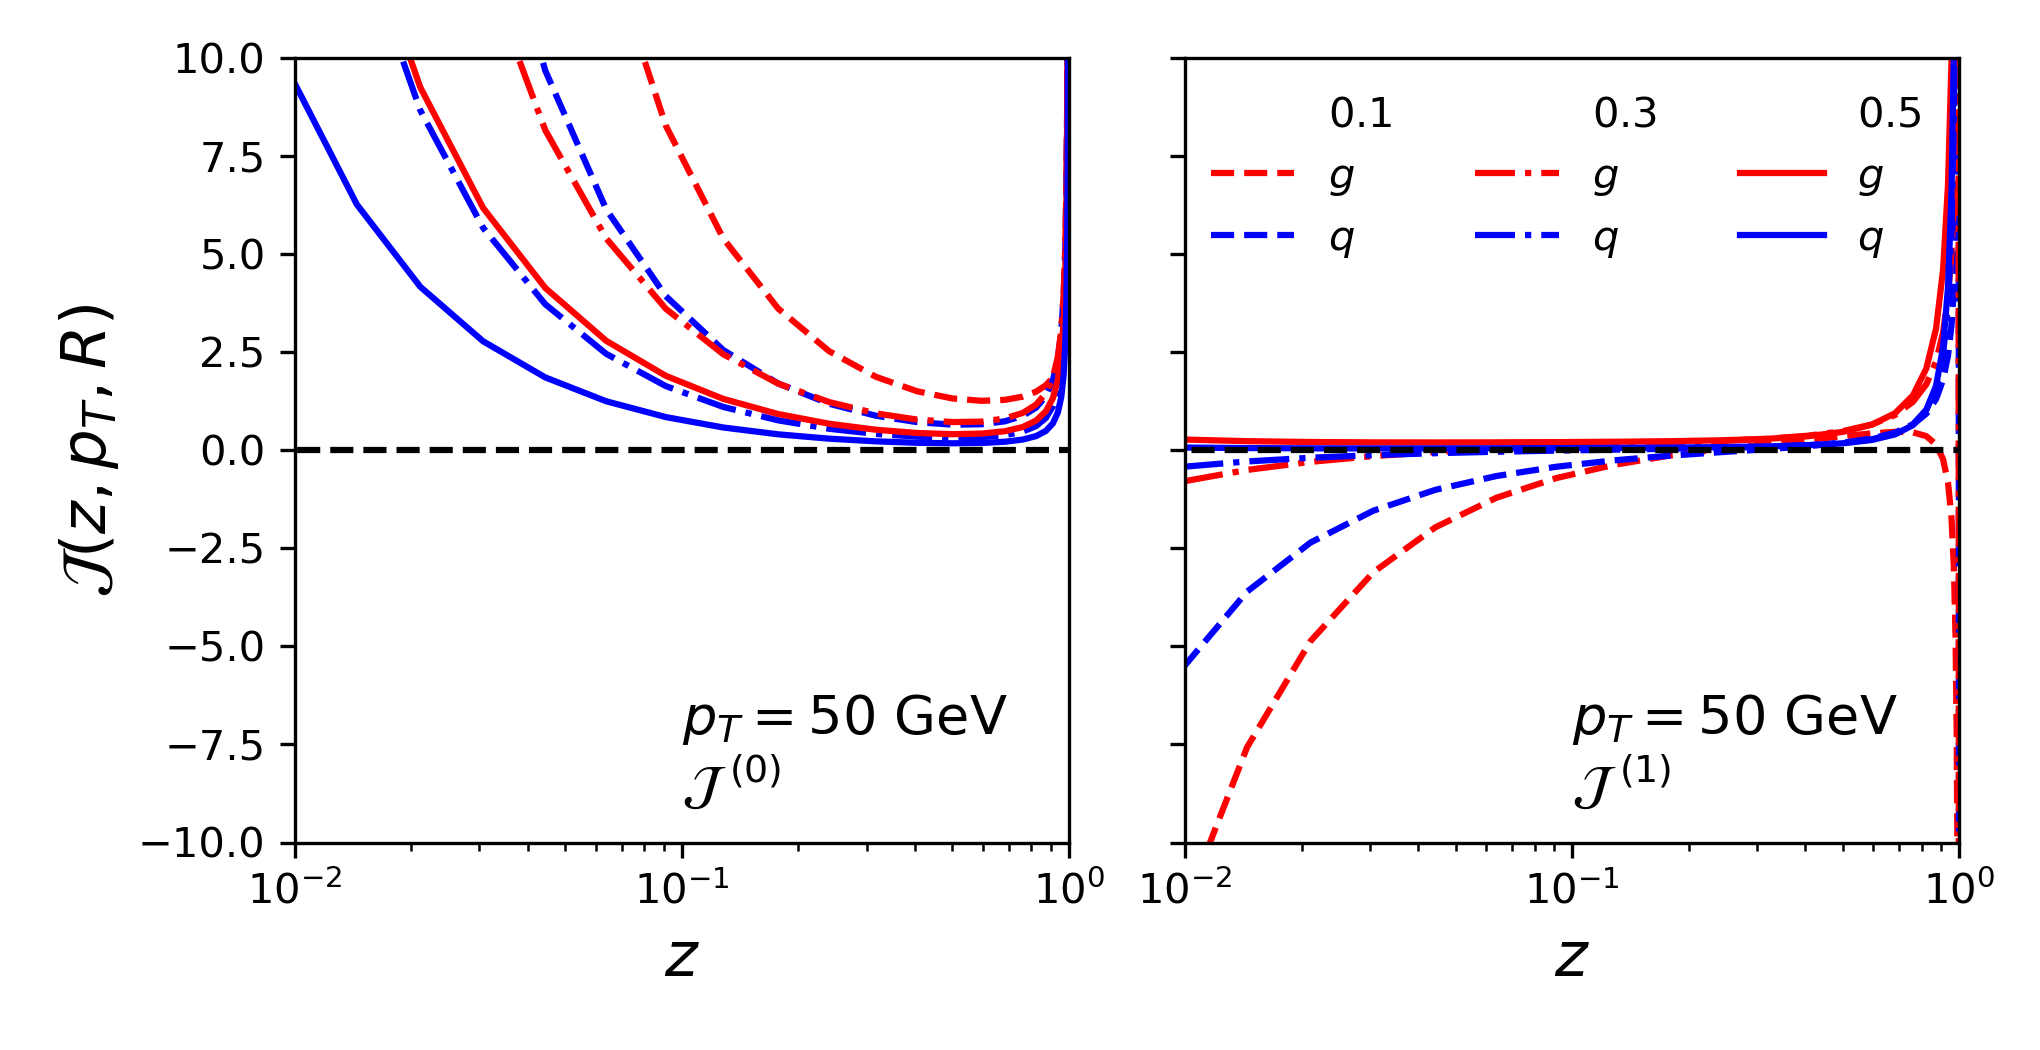
\includegraphics[width=.8\textwidth]{JetFunctions-R.png}
\end{center}

\begin{itemize}
\item $\mathcal{J}^{(0)}$ agree with Zhong-Bo Kang, Felix Ringer and Ivan Vitev 1606.06732.
\item  $\mathcal{J}^{(1)}$ qualitatively similar, but quantiatively different form 1606.06732. I suspect it to be the number of active flavor $N_f$ one assumes.
\end{itemize}

\end{frame}

\begin{frame}{Numerical check of inclusive jet cross section}

\vskip1em
\begin{columns}
\begin{column}{.5\textwidth}
ATLAS, 7 TeV, $R=0.4$ 1410.8857

\begin{center}
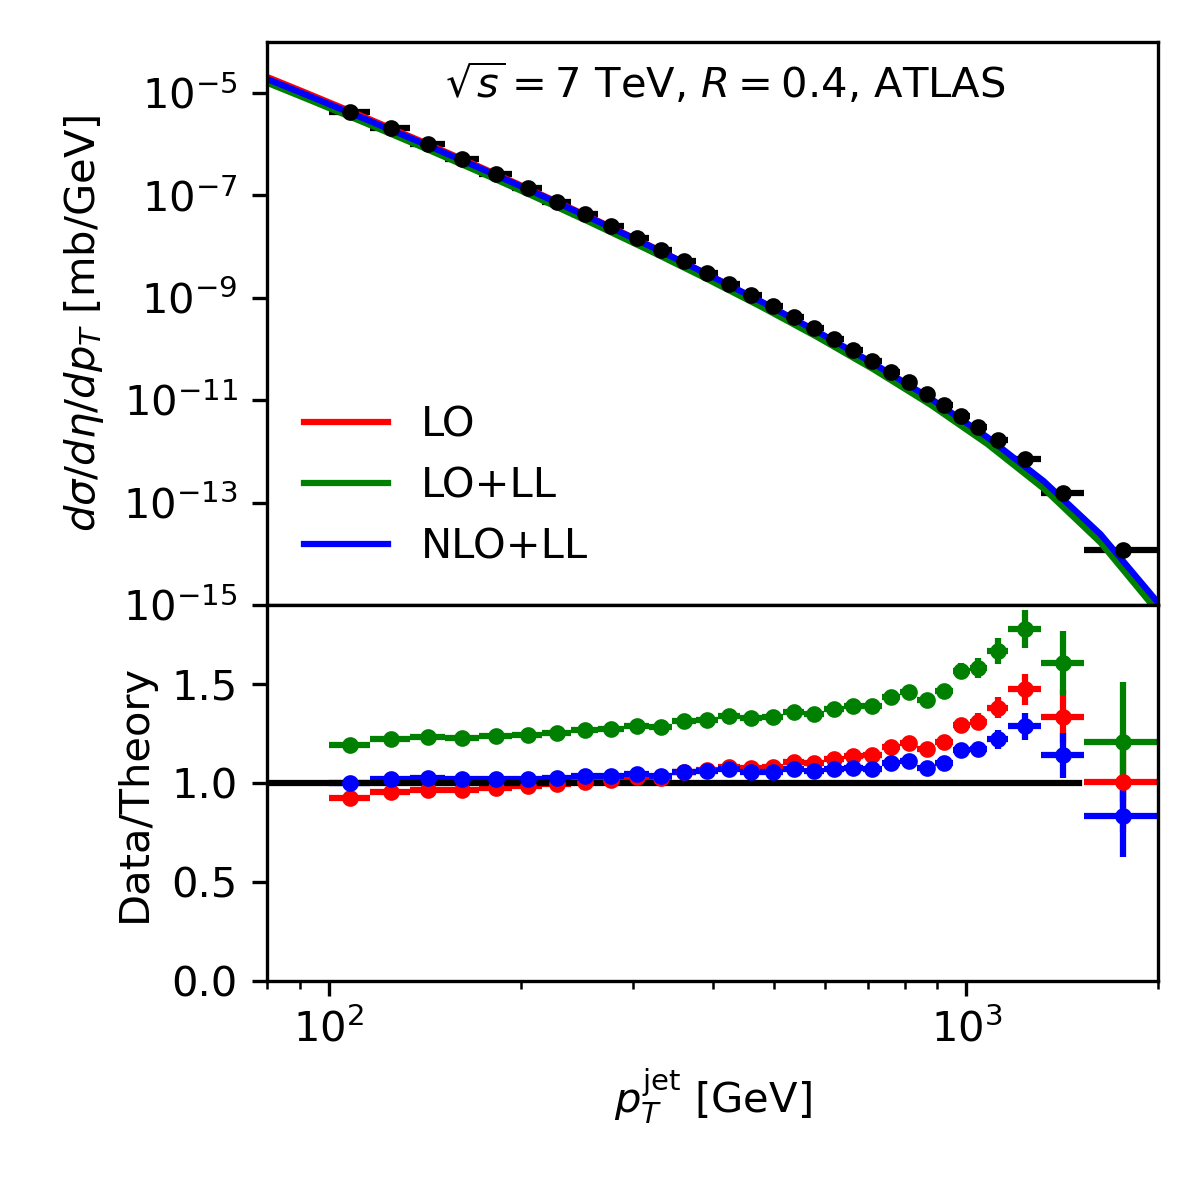
\includegraphics[width=\textwidth]{ATLAS-jet-R0d4.png}
\end{center}
\end{column}

\begin{column}{.5\textwidth}
STAR, 0.2 TeV, $R=0.4$ hep-ex/0608030

\begin{center}
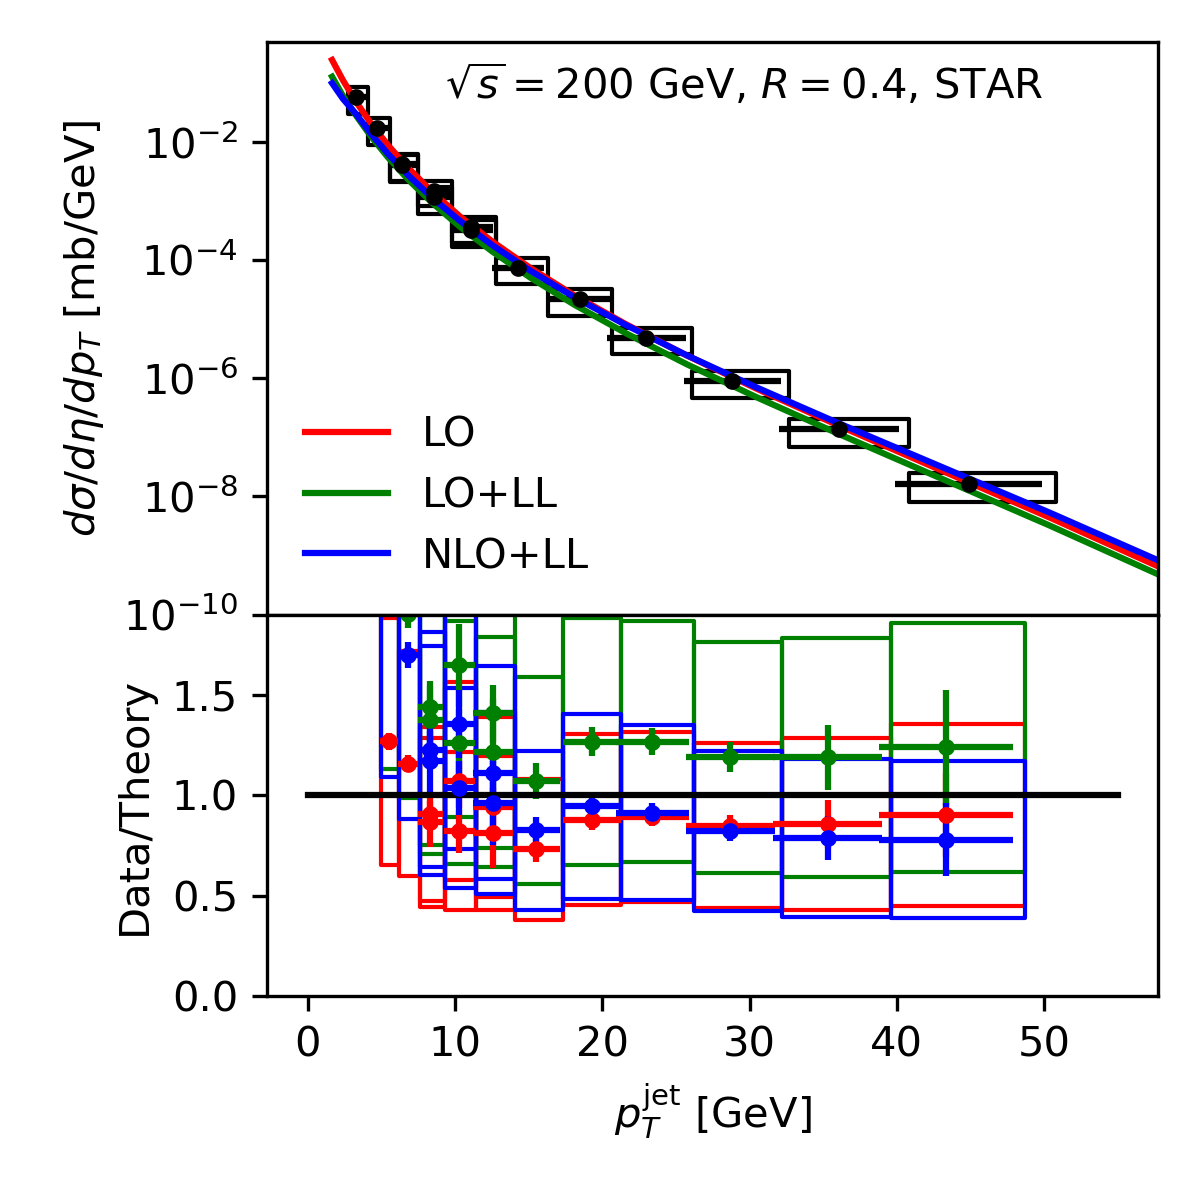
\includegraphics[width=\textwidth]{STAR-jet-R0d4.png}
\end{center}
\end{column}

\end{columns}
\end{frame}

\begin{frame}{Numerical check of inclusive jet cross section}

\vskip1em
ALICE, 5.02 TeV, 1909.09718
\vskip1em
\begin{columns}
\begin{column}{.33\textwidth}
 $R=0.1$ 

\begin{center}
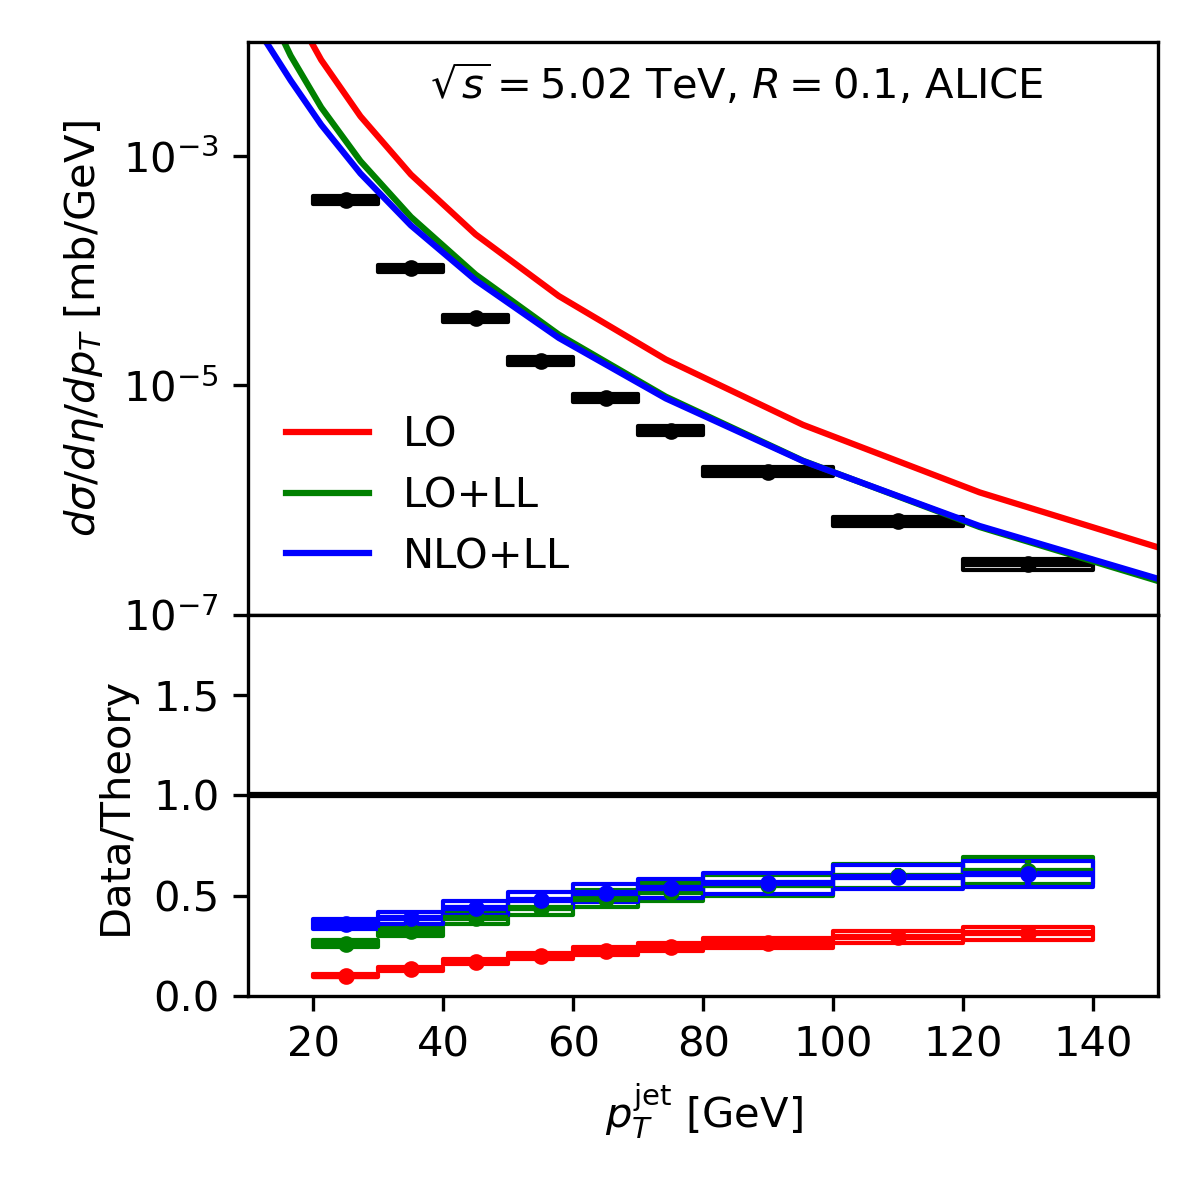
\includegraphics[width=\textwidth]{ALICE-jet-R0d1.png}
\end{center}
\end{column}

\begin{column}{.33\textwidth}
 $R=0.2$ 

\begin{center}
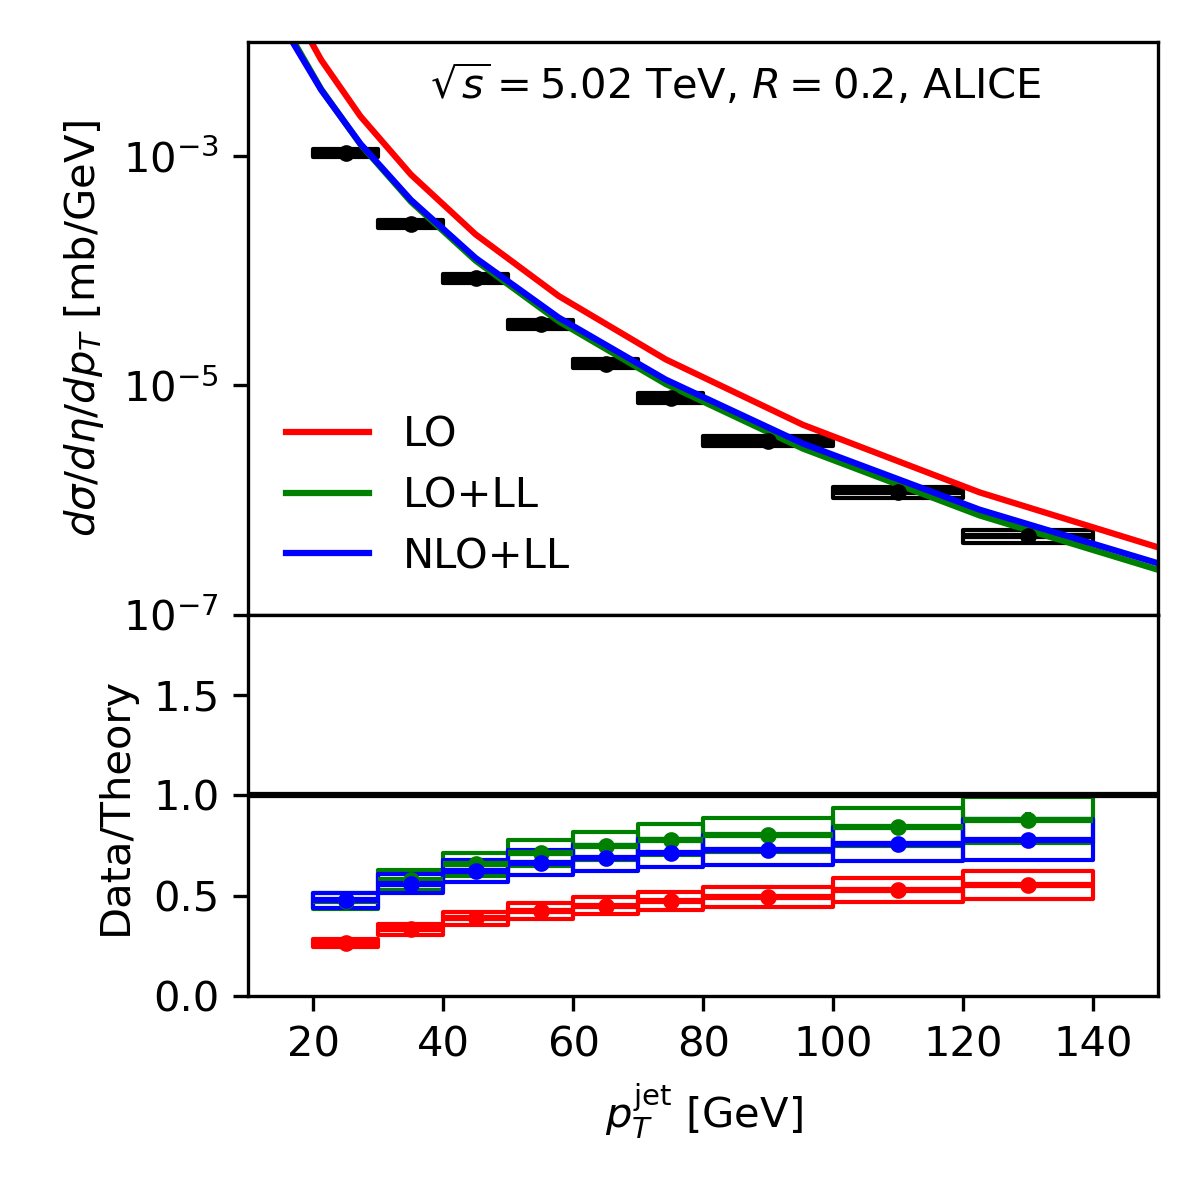
\includegraphics[width=\textwidth]{ALICE-jet-R0d2.png}
\end{center}

\end{column}

\begin{column}{.33\textwidth}
 $R=0.4$ 

\begin{center}
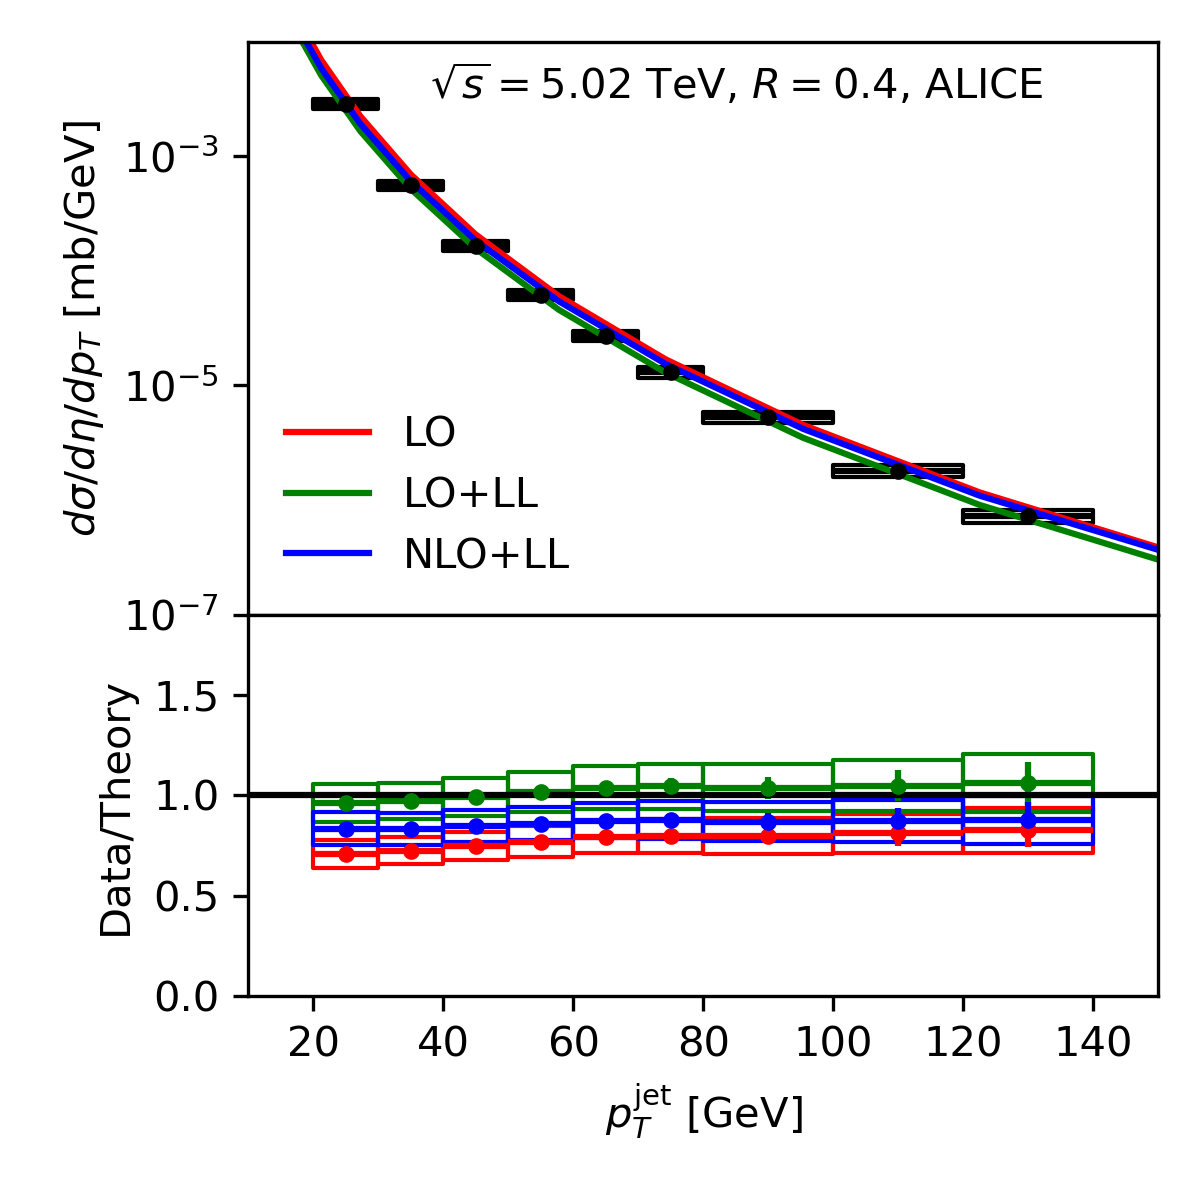
\includegraphics[width=\textwidth]{ALICE-jet-R0d4.png}
\end{center}

\end{column}

\end{columns}
\end{frame}

\begin{frame}{Numerical check of inclusive jet cross section}

\vskip1em
CMS, 2.76 TeV, 1609.05383
\vskip1em
\begin{columns}
\begin{column}{.33\textwidth}
 $R=0.2$ 

\begin{center}
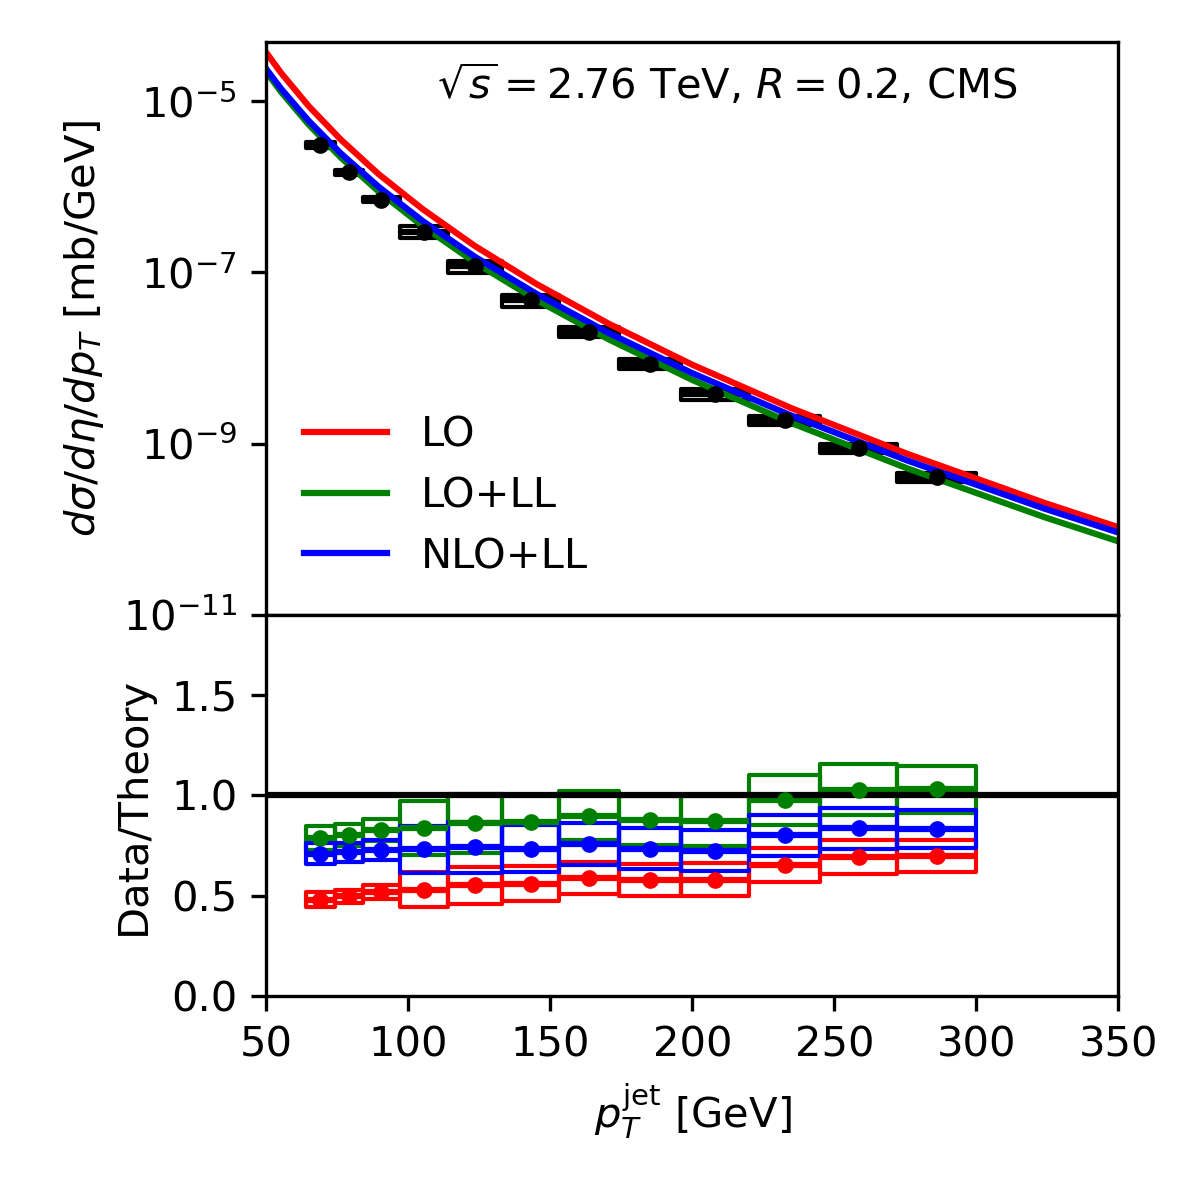
\includegraphics[width=\textwidth]{CMS-jet-R0d2.png}
\end{center}
\end{column}

\begin{column}{.33\textwidth}
 $R=0.3$ 

\begin{center}
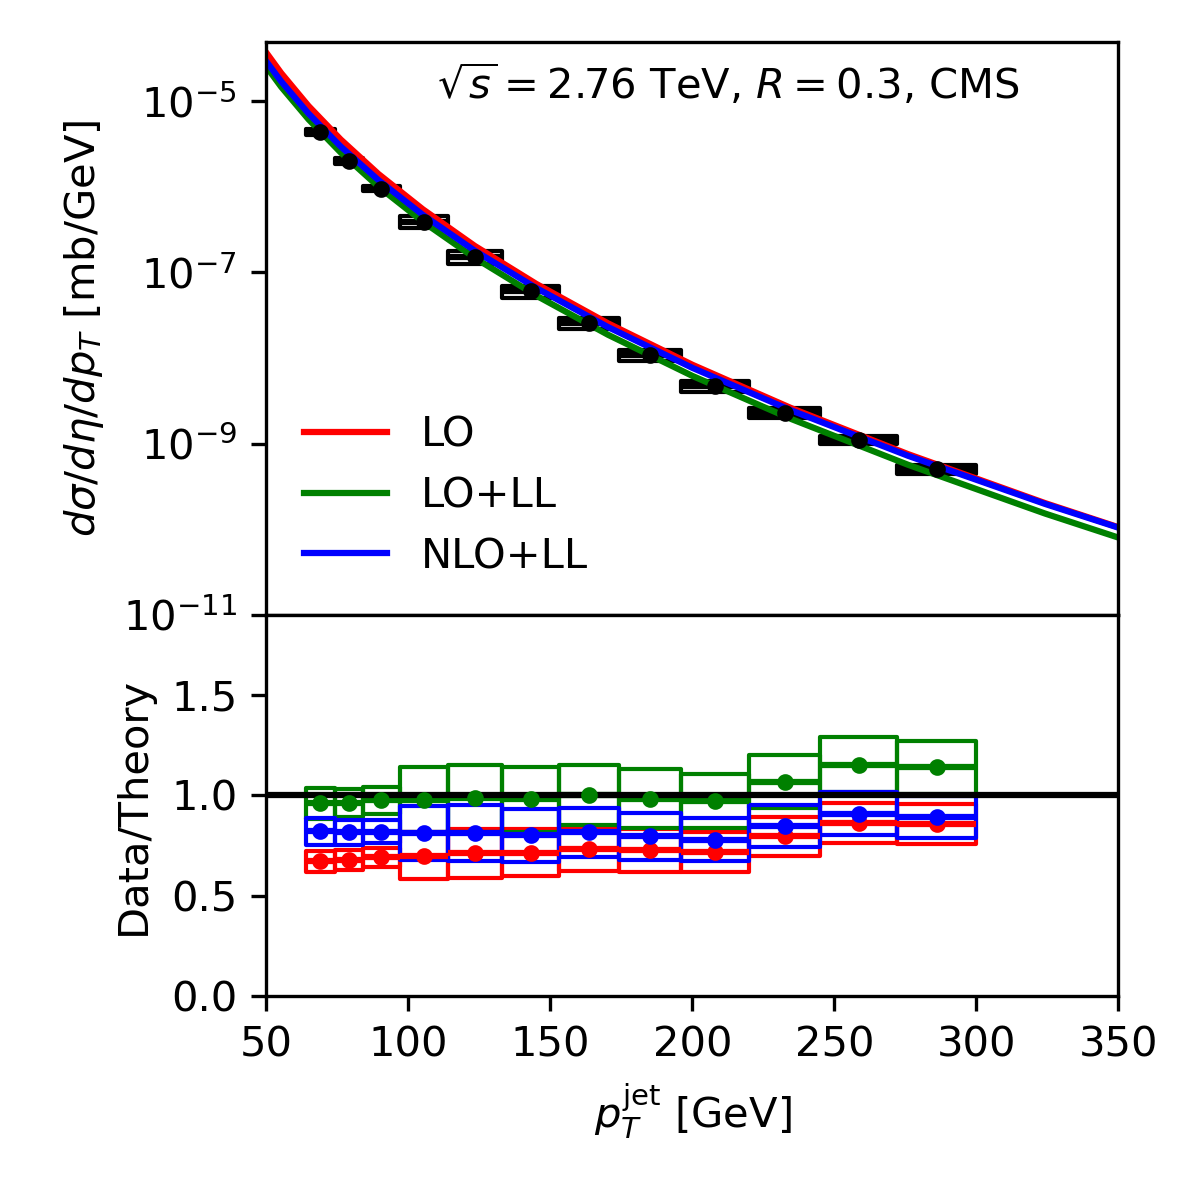
\includegraphics[width=\textwidth]{CMS-jet-R0d3.png}
\end{center}

\end{column}

\begin{column}{.33\textwidth}
 $R=0.4$ 

\begin{center}
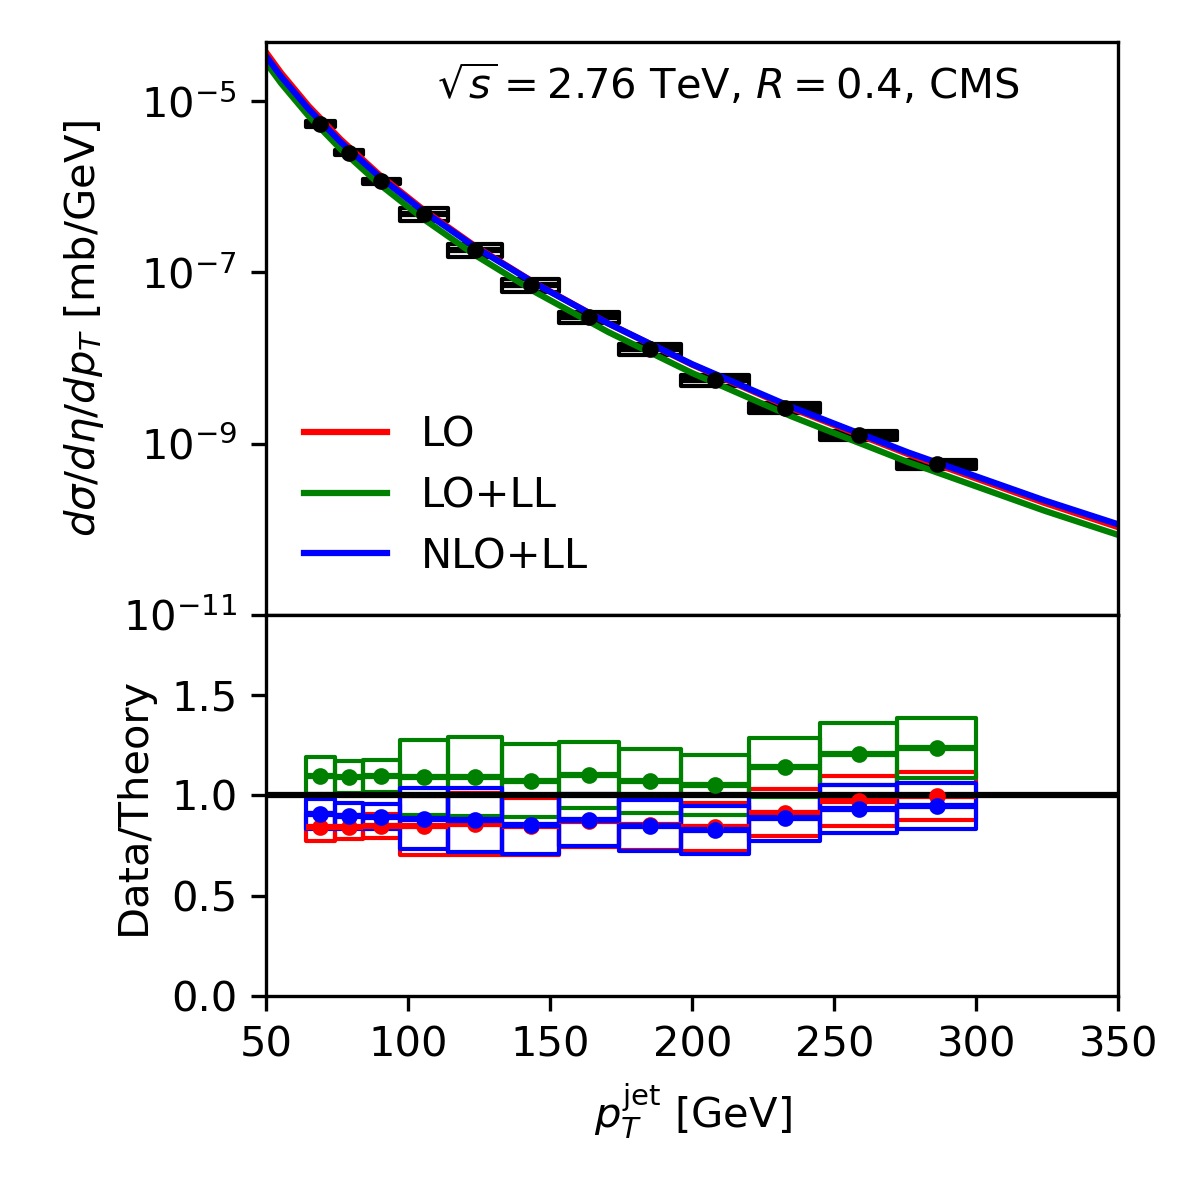
\includegraphics[width=\textwidth]{CMS-jet-R0d4.png}
\end{center}

\end{column}

\end{columns}
\end{frame}


\end{document}